\documentclass[12pt]{article}
\usepackage[letterpaper, portrait, margin=.5in]{geometry}
\usepackage[T1]{fontenc}
%\usepackage{lmodern}
\usepackage[letterspace=-50]{microtype}
\usepackage[dvipsnames]{xcolor}
\usepackage{pgfplots}
\pgfplotsset{compat=1.8}
\usepackage{multicol}
\usepackage{eso-pic}
\definecolor{primary}{HTML}{de4f4f}
\definecolor{secondary}{HTML}{2b2e39}
\definecolor{accent}{HTML}{e0e0e0}
\def\labelitemi{--}
\def\columnseprulecolor{\color{secondary}}
%\renewcommand{\rmdefault}{bookman}

\pagecolor{secondary}
\AddToShipoutPictureBG{
  \AtPageLowerLeft{%
    \color{accent}%
    \rule{\pdfpagewidth}{\dimexpr\pdfpageheight-3.8in}%
  }
}


\setlength{\columnseprule}{4pt}
\newcommand{\tab}[1]{\hspace{.1\textwidth}\rlap{#1}}

\begin{document}
\sffamily
\lsstyle
\color{white}
\center
\begin{Huge}\textbf{Bryce John Sampson}\end{Huge}\\
\medskip
\fontsize{12}{1.2}
\selectfont
\smallbreak
\colorbox{accent}{
    \parbox{45em}{
        \centering
        \color{secondary}
        sampson.bryce@yahoo.com | +1 530-859-5330 | 605 West 6th Street Chico, CA 95926 \\
        \large
        \textbf{\color{primary}www.brycethebuilder.com |}
        \textbf{\color{primary}www.github.com/sampsonbryce}
    }
}
\smallskip
\center
\textbf{\Large------ Education ------}\\
\flushleft
\begin{footnotesize}
\textsc{California State University, Chico CA}
\hfill
\textbf{\color{primary}Major GPA: }3.95\\

\smallskip
\textsc{Linnaeus University, Vaxjo Sweden (2017-18 Year Abroad)}
\hfill
\textbf{\color{primary}Cumulative GPA: }3.77\\
\smallskip

{\color{accent}Expected Graduation Spring 2019}
\hfill
\textbf{\color{primary}Major: }Computer Science\\
\smallskip

\end{footnotesize}

\colorbox{primary}{
\parbox{45.5em}{
    \color{secondary}
    \begin{multicols}{2}
    \begin{center}
    \textbf{\color{white}\large Proficiency}
    \bigbreak
    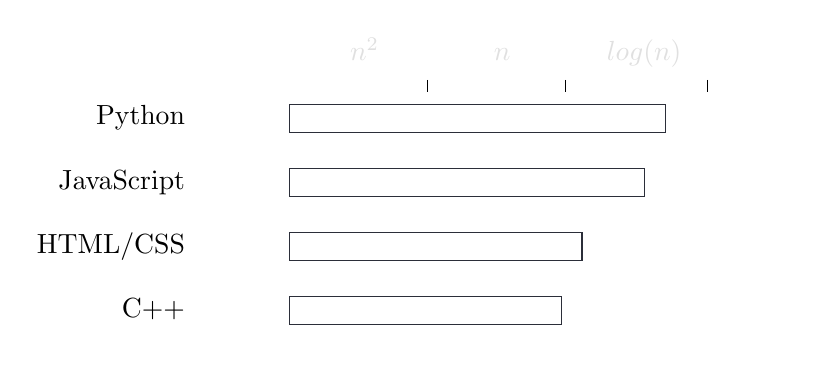
\begin{tikzpicture} 
        \begin{axis}[
        height=5cm,
        width = 9cm,
        xbar,
        xmin=0,
        xmax=100,
        xtick={33,66,100},
        xticklabels = {$n^2$, $n$, $log(n)$},
        y axis line style = { opacity = 0 },
        ytick             = data,
        typeset ticklabels with strut, % improves vertical alignment of some of the ticklabels in this case (compare gcc and mcf with and without)
        ytick style = {draw=none},
        xtick pos=top,
        every x tick/.style={black},
        every x tick label/.append style={accent},
        xticklabel style = {xshift=-.8cm},
        enlarge y limits  = 0.2,
        enlarge x limits  = 0.2,
        symbolic y coords = {C++,HTML/CSS,JavaScript,Python},
        ]
        \addplot[secondary!20!secondary,fill=white!80!white] coordinates {(70,HTML/CSS)(90,Python)(85,JavaScript)(65,C++)};
        \end{axis} 
    \end{tikzpicture}
    \smallbreak
    \footnotesize
    \color{secondary}Git | Vim | Linux | Windows | MacOS | Android
    \end{center}
    \columnbreak
    \center
    \footnotesize
    \textbf{\color{white}\normalsize ACM Club | CSU, Chico}\\
    \smallskip
    {\color{accent}Algorithms Officer} \hfill \textit{\color{accent}Spring 2017}\\
    \begin{itemize}
    \setlength{\itemsep}{0pt}
        \item Competed in Fall 2016 ACM Competition
        \item Research and present/teach algorithms at club meetings to be used during competition
    \end{itemize}

    \center
    \textbf{\color{white} 
        \normalsize
        Formula SAE Electric | CSU, Chico
    }\\
    
    \smallskip
    {\color{accent}Member} \hfill \textit{\color{accent}Spring 2017}

    \begin{itemize}
    \setlength{\itemsep}{0pt}
        \item Develop Formula SAE car to compete nationally
        \item Contribute to batteries and motor control team
    \end{itemize}


    \end{multicols}
}}
    \color{secondary}
    \center
    \begin{center}
    \textbf{\Large------ Internships ------}\\
    \end{center}
    \begin{footnotesize}
    \flushleft
    \textbf{\color{primary}\large Workday Inc} \hfill \textbf{\color{Cerulean}Python | Bash}\\ 
    {\color{primary}4 months | full-time | May - August 2017} \hfill {\color{Cerulean} Environment Engineer Intern}
    \vspace{-2mm}
    \begin{itemize}
        \setlength{\itemsep}{0pt}
        \item Developed internal environment management tools for Automation and Network Operations sub-team of the Environments department
        \item Provisioned and de-provisioned environments for Sales Environment team
    \end{itemize}
    \textbf{\color{primary}\large SocialHighRise} \hfill  \textbf{\color{Cerulean}HTML/CSS/JS | jQuery | ASP.NET MVC | C\# | Razor | WordPress } \\ 
    {\color{primary}10 months | part-time | August 2016 - May 2017} \hfill {\color{Cerulean} Software Development Intern}
    \vspace{-2mm}
    \begin{itemize}
        \setlength{\itemsep}{0pt}
        \item Develop in-house account manangement tool for organizing and monitoring social media profiles
        \item Manage all company tech support and IT needs including company website development
    \end{itemize}
    \textbf{\color{primary}\large Lawrence Livermore National Laboratory} \hfill \textbf{\color{Cerulean}PySide Qt | Python | HTML/CSS/JS | jQuery | React/Redux}\\
    {\color{primary}8 months | full-time | January - August 2016} \hfill {\color{Cerulean} Computation Intern}
    \vspace{-2mm}
    \begin{itemize}
        \setlength{\itemsep}{0pt}
        \item Employed in a Co-op position, developing a Graphical User Interface for a large scale climate data visualization and analysis tool developed at the lab.
        \item Developed GUI in both PySide Qt and from scratch in HTML/CSS/JS, jQuery, React/Redux, and Flask

        \item Organized and presented demos of project to our team and communicated development timeline
        \item Collaborated with scientists using alpha, beta and previous versions of GUI to improve user experience and implement new functionality
    \end{itemize}

    \end{footnotesize}
    
\colorbox{secondary}{
    \parbox{45em}{
    \color{white}
    \begin{center}
    \textbf{\Large------ Projects ------}\\
    \end{center}
    \begin{footnotesize}

    \textbf{\color{primary}\large Hero Home (www.home.heroinc.io):} \hfill \textbf{\color{Cerulean}Vue.js | HTML/CSS | Node.js/Express | Nginx }
    \begin{itemize}
        \item Chrome Extension and Home Page for Google search that displays advertisements to raise money for charity
    \end{itemize}


    \flushleft

    \textbf{\color{primary}\large Datasift Sentiment Visualization:} \hfill \textbf{\color{Cerulean} Node.js/Express | React | D3 | HTML/CSS/JS | jQuery}
    \begin{itemize}
        \item Utilized Datasift Facebook Topic Data API trial to create visualization representing sentiment 
    \end{itemize}

    \end{footnotesize}
}}

\center
Created with \LaTeX
\end{document}
